\section{Introduction}\label{intro}

WebAssembly (Wasm)~\cite{haas2017bringing} is a popular binary
instruction format that enables the execution of untrusted code in a
safe, isolated environment. Moreover, it is a portable compilation
target for different languages, and can be executed efficiently on a
wide range of platforms without the need of dedicated hardware. Wasm
was originally meant to be run inside web browsers, but given the
considerable advantages it brings, many runtimes that allow
execution in standalone mode have been developed recently. Popular
examples are Wasmtime, WasmEdge, Wasmer, and WAMR.

To answer the developers' need to access resources of the host
system from within the runtime, a standardization effort called
WebAssembly System Interface (WASI)~\cite{wasi} is undergoing.
Its goal is to provide a stable and multi-platform system interface. To be WASI-compliant, each runtime must implement
all the calls defined in the interface with dedicated functions, which
are named hostcalls. However, implementing these functions is
non-trivial, since (i) the code must not introduce violations to the
Wasm memory model, and (ii) it is possible to break the separation
between the system and the isolated environment in which the Wasm module is
executed. The solution adopted by current runtimes leverages
WASI Libc~\cite{wasi-libc}, a library providing POSIX-compatible APIs
built on top of hostcalls.

% The first proposal of a system interface was the file system one.
Currently, every WASI-compliant runtime implements the proposed file system
interface with a libpreopen-like layer~\cite{libpreopen}. Whenever the runtime
receives a request to open a file, it first checks whether the path
belongs to the authorized list of directories, then it opens the file
on behalf of the Wasm program, redirecting the content to the caller.
Previous work~\cite{johnson2022wave,
  bosamiya2022provably, lehmann2020everything} proved the approach
to be error-prone, leaving the system unprotected when a vulnerability
was introduced in a hostcall wrapper (Figure~\ref{fig:wasi}). Moreover,
this approach provides limited flexibility, as it is associated with
directory-based granularity instead of file-based. Lastly, in order to audit
the policy regulating resource access, one must find the permissions
by looking at the code.
We claim that there is no practical advantage in having several
implementations of the same access control checks for different
runtimes. Our idea is to replace the user-space runtime-specific
security checks with a single in-kernel implementation that leverages
eBPF~\cite{bpf-lsm-hooks}.
There are considerable advantages in doing so: (i)~it permits to decouple the implementation of hostcall wrappers
and the access control details, minimizing the risk of bugs~\cite{kehoe2022ebpf,seapp, cage4deno},
(ii)~it enables the introduction of per-module policies with file-based
granularity, and (iii)~it fulfills Wasm's promise of portability as eBPF programs are portable across different kernel versions~\cite{andrii2021bpfCORE} and also operating systems, thanks
to Microsoft's undergoing effort to port eBPF to
Windows~\cite{ebpf-windows}.
% In the following we describe the threat model and our efforts to
% integrate eBPF into production Wasm runtimes. Finally, we discuss
% our results.

\section{Threat model}

Our assumptions reflect the threat model employed by Wasm runtimes. We
assume that the code executed by the runtime is either untrusted or it
is trusted but potentially affected by security vulnerabilities due to
bugs. The goal of the attacker providing the code is to bypass the
security checks enforced by the runtime to get access to the host file
system. To fulfill this objective, the attacker can leverage the
interface provided by WASI and send any argument. Runtime escapes
caused by memory corruption or alteration of the program flow are out
of scope of our work, since protection can be provided by other
existing solutions (e.g., ~\cite{bosamiya2022provably}).

\begin{figure}[t!]
	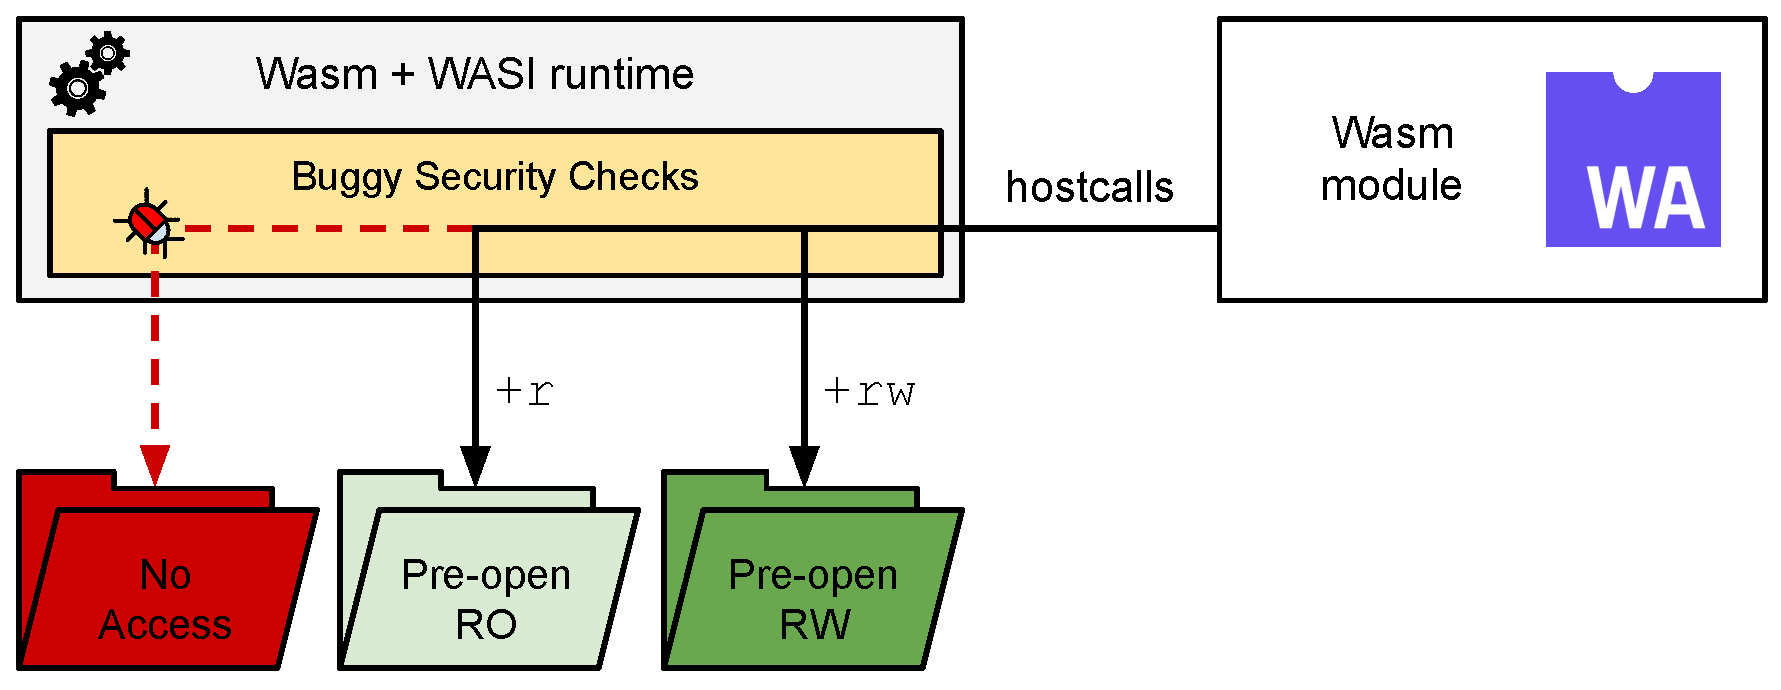
\includegraphics[width=\columnwidth]{chapters/wasm/fig/wasi}
	\caption[Current implementation of WASI by runtimes]{
    Current implementation of WASI by runtimes. A bug present in a
    hostcall wrapper permits the module to read the unauthorized
    directory on the left (red dotted arrow)
  }
	\label{fig:wasi}
\end{figure}


%%% Local Variables:
%%% mode: latex
%%% TeX-master: "../main.tex"
%%% End:
